Like GWT \citep{modflow6gwt}, the GWE Model simulates three-dimensional transport in flowing groundwater.  The primary difference between GWT and GWE is that heat (i.e., temperature), instead of concentration, is the simulated ``species.'' As such, the GWE Model solves the heat transport equation using numerical methods and a generalized control-volume finite-difference approach, which can be used with regular MODFLOW grids (DIS Package) or with unstructured grids (DISV and DISU Packages).  The GWE Model is designed to work with most of the new capabilities released with the GWF Model, including the Newton flow formulation, XT3D \citep{modflow6xt3d}, unstructured grids, advanced packages, and the movement of water between packages.  The GWF and GWE (and, if active, GWT) models operate simultaneously during a \mf simulation to represent coupled groundwater flow and heat transport.  The GWE Model can also run separately from a GWF Model by reading the heads and flows saved by a previously run GWF Model.  The GWE model is also capable of working with the flows from another groundwater flow model as long as the cell-by-cell and boundary flows and groundwater heads are written to ``linker'' files in the correct format.  

The purpose of the GWE Model is to calculate changes in groundwater temperature in both space and time.  Groundwater temperature within an aquifer can change in response to different energy transport processes.  These processes include (1) convective (advective) transport of heat with flowing groundwater, (2) the combined hydrodynamic dispersion processes of velocity-dependent mechanical dispersion and conduction (analogous to chemical diffusion), (3) thermal equilibrium with the aquifer matrix, (4) mixing of fluids from groundwater sources and sinks, and (5) direct addition of thermal energy.

For GWE, the temperature at any point in the aquifer is assumed to instantaneously equilibrate between the aqueous and solid phase domains.  For example, a pulse of heat convecting through an aquifer will be retarded through thermal equilibration with the aquifer material.  Conversely, the introduction of cold groundwater into a previously warm region of the aquifer will warm up, at least in part, as energy within the aquifer matrix transfers to the aqueous phase.  Unlike GWT, the GWE Model type does not support an immobile domain.  The energy that is transferred between the aqeous and solid phases of the groundwater system are tracked in the GWE Model budget.

This section describes the data files for a \mf Groundwater Energy Transport (GWE) Model.  A GWE Model is added to the simulation by including a GWE entry in the MODELS block of the simulation name file.  There are three types of spatial discretization approaches that can be used with the GWE Model: DIS, DISV, and DISU.  The input instructions for these three packages are not described here in this section on GWE Model input; input instructions for these three packages are described in the section on GWF Model input.

The GWE Model is designed to permit input to be gathered, as it is needed, from many different files.  Likewise, results from the model calculations can be written to a number of output files. The GWE Model Listing File is a key file to which the GWE model output is written.  As \mf runs, information about the GWE Model is written to the GWE Model Listing File, including much of the input data (as a record of the simulation) and calculated results.  Details about the files used by each package are provided in this section.

The GWE Model reads a file called the Name File, which specifies most of the files that will be used in a groundwater energy transport simulation. Several files are always required whereas other files are optional depending on the question(s) being addressed by the model. The Output Control Package receives instructions from the user to control the amount and frequency of output.  Details about the Name File and the Output Control Package are described in this section.

For the GWE Model, ``flows'' (unless stated otherwise) represent the ``flow'' of energy, often expressed in units of energy (e.g., joules) per time, rather than groundwater flow.  

\subsection{Information for Existing Heat Transport Modelers}
An important goal of the \mf GWE Model is to alleviate the need for ``parameter equivalents'' when simulating heat transport in groundwater systems.  In the past, codes like HST3D \citep{kipp1987} or VS2DH \citep{healy1996} simulated energy transport directly by supporting the use of native heat transport units.  For example, users could directly specify thermal conductivity of the fluid and solid phases, as well as the heat capacity of both phases.  Alternatively, codes like MT3DMS \citep{zheng1999mt3dms}, MT3D-USGS \citep{mt3dusgs}, and MODFLOW-USG \citep{modflowusg} could be used to simulate the movement of heat in groundwater, but required users to leverage existing variables as surrogates for heat transport.  For example, the molecular diffusion parameter may be used as a surrogate for simulating thermal conduction in an aquifer \citep{mazheng2010, hechtmendez}. 

The following list summarizes important aspects of GWE for simulating heat transport with \mf:

\begin{enumerate}

\item The GWE Model uses parameters that are native to heat transport, including thermal conductivity of water, heat capacity of water, thermal conductivity of the aquifer material, heat capacity of of the aquifer material, and latent heat of vaporization. Therefore, users do not need to pre-calculate solute-transport ``parameter equivalents'' when generating GWE model input; users can instead enter native parameter values that are readily available.

\item Thermal energy transport budgets written to the \mf list file are reported in units of energy (e.g., joules).  Previously, using a program like MT3D-USGS \citep{mt3dusgs} to emulate heat transport using solute transport, units in the list file budget did not correspond to thermal energy, but were reported in units of $\frac{m^{3 \;\circ}C}{d}$. To convert to thermal energy units, values in the list file had to be post-processed by multiplying each line item by the density of water ($\rho_w$) and the heat capacity of water ($C_p$) \citep{langevin2008seawat}.

\item Thermal equilibrium between the aqueous and solid phases is assumed.  Thus, simulated temperatures are representative of both phases.  As a result, thermal conduction between adjacent cells may still occur even in the absence of convection.

\item In GWE, dry cells (devoid of groundwater) remain active for simulating thermal conduction. For example, energy (heat) transfer will be simulated between a partially saturated cell (i.e., ``water-table'' cell) and an overlying dry cell. In this way, a more full accounting of various heat transport processes is represented in the subsurface.  Moreover, this approach readily supports heat transport in the unsaturated-zone when the UZE (unsaturated-zone energy transport) Package is active.  

\item Heat transport is supported for all five of the advanced GWF packages using the following packages in GWE: (1) streamflow energy transport, SFE Package; (2) lake energy transport, LKE Package; (3) multi-aquifer well energy transport, MWE Package; (4) unsaturated zone energy transport, UZE Package; and the (5) Water Mover Package, MVE.  Similar to GWT, GWE will simulate heat transfer between an advanced package and the groundwater system via groundwater surface-water exchange; however, GWE also simulates a conductive transfer of heat between an advanced package feature and the aquifer.  To take advantage of this functionality, users must specify the thermal conductivity of the material separating a stream from the aquifer, for example, the thermal conductivity of the streambed (or lakebed), as well as the thickness of the streambed (or lakebed).  As with the advanced GWT packages, GWE simulates thermal convection between package features, such as between two stream reaches for example.  Also, dispersive heat transport among among advanced package features is not represented, similar to GWT.

\item Where the GWF model simulates evaporation from an open body of water, for example from the surface of a stream or lake, the latent heat of vaporization may be used to simulate evaporative cooling.  As water is converted from liquid to gas, the energy required by the phase change is drawn from the remaining body of water and the resulting cool down is calculated.

\end{enumerate}

Many of the same considerations listed for the GWT model should be kept in mind when developing a GWE model. For convenience, many of those considerations are adapted for GWE and repeated here.

\begin{enumerate}

\item A GWE Model can access flows calculated by a GWF Model that is running in the same simulation as the GWE Model.  Alternatively, a GWE Model can read binary head and budget files created from a previous GWF Model simulation (provided these files contain all of the required information for all time steps); there is no specialized flow and transport link file \citep{zheng2001modflow} as there is for MT3D.  Details on these two different use cases are provided in the chapter on the FMI Package.

\item The GWE Model is based on a generalized control-volume finite-difference method, which means that heat transport can be simulated using regular MODFLOW grids consisting of layers, rows, and columns, or heat transport can be simulated using unstructured grids.

\item GWE and GWT use the same advection package source code.  As a result, advection can be simulated using central-in-space weighting, upstream weighting, or an implicit second-order TVD scheme.  Currently, neither the GWE or GWT models can use a Method of Characteristics (particle-based approaches) or an explicit TVD scheme to simulate convective (or advective) transport.  Consequently, the GWE Model may require a higher level of spatial discretization than other transport models that use higher order terms for advection dominated systems.  This can be an important limitation in problems involving sharp heat fronts. 

\item The Viscosity Package can use temperatures from the GWE model to adjust the viscosities in the flow model.   

\item GWE and GWT use the same Source and Sink Mixing (SSM) Package for representing the effects of GWF stress package inflows and outflows on simulated temperatures and concentrations.  In a GWE simulation, there are two ways in which users can assign temperatures to the individual features in these stress package.  The first way is to activate a temperature auxiliary variable in the corresponding GWF stress package.  In the SSM input file, the user provides the name of the auxiliary variable to be used for temperature.  The second way is to create a special SPC file, which contains user-assigned time-varying temperatures for stress package features.

\item The GWE model includes an Energy Storage and Transfer (EST) Package that is analogous to the MST Package in the GWT Model.  The GWE Model does not simulate immobile domains and therefore does not include an analog of the IST Package in the GWT Model.  

\item A GWE-GWE Exchange (introduced in version 6.5.0) can be used to tightly couple multiple heat transport models, as might be done in a nested grid configuration.  

\item There is no option to automatically run the GWE Model to steady state using a single time step.  This is an option available in MT3DMS \citep{zheng2010supplemental}.  Steady state conditions must be determined by running the transport model under transient conditions until temperatures stabilize.

\item As is the case with GWT, the GWE Model has not yet been programmed to work with the Skeletal Storage, Compaction, and Subsidence (CSUB) Package for the GWF Model.  

\end{enumerate}

\subsection{Units of Length and Time}
The GWE Model formulates the groundwater energy transport equation without using prescribed length and time units. Any consistent units of length and time can be used when specifying the input data for a simulation. This capability gives a certain amount of freedom to the user, but care must be exercised to avoid mixing units.  The program cannot detect the use of inconsistent units.

\subsection{Thermal Energy Budget}
A summary of all inflow (sources) and outflow (sinks) of thermal energy is referred to as an energy budget.  \mf calculates an energy budget for the overall model as a check on the acceptability of the solution, and to provide a summary of the sources and sinks of energy to the flow system.  The energy budget is printed to the GWE Model Listing File for specified time steps.

\subsection{Time Stepping}

For the present implementation of the GWE Model, all terms in the heat transport equation are solved implicitly.  With the implicit approach applied to the transport equation, it is possible to take relatively large time steps and efficiently obtain a stable solution.  If the time steps are too large, however, accuracy of the model results will suffer, so there is usually some compromise required between the desired level of accuracy and length of the time step.  An assessment of accuracy can be performed by simply running simulations with shorter time steps and comparing results.

In \mf time step lengths are controlled by the user and specified in the Temporal Discretization (TDIS) input file.  When the flow model and heat transport model are included in the same simulation, then the length of the time step specified in TDIS is used for both models.  If the GWE Model runs in a separate simulation from the GWE Model, then the time steps used for the heat transport model can be different, and likely shorter, than the time steps used for the flow solution.  Instructions for specifying time steps are described in the TDIS section of this user guide; additional information on GWF and GWE configurations are in the Flow Model Interface section.  



\newpage
\subsection{GWE Model Name File}
The CHF Model Name File specifies the options and packages that are active for a CHF model.  The Name File contains two blocks: OPTIONS  and PACKAGES. The lines in each block can be in any order.  Files listed in the PACKAGES block must exist when the program starts. 

Comment lines are indicated when the first character in a line is one of the valid comment characters.  Commented lines can be located anywhere in the file. Any text characters can follow the comment character. Comment lines have no effect on the simulation; their purpose is to allow users to provide documentation about a particular simulation. 

\vspace{5mm}
\subsubsection{Structure of Blocks}
\lstinputlisting[style=blockdefinition]{./mf6ivar/tex/chf-nam-options.dat}
\lstinputlisting[style=blockdefinition]{./mf6ivar/tex/chf-nam-packages.dat}

\vspace{5mm}
\subsubsection{Explanation of Variables}
\begin{description}
\input{./mf6ivar/tex/chf-nam-desc.tex}
\end{description}

\begin{table}[H]
\caption{Ftype values described in this report.  The \texttt{Pname} column indicates whether or not a package name can be provided in the name file.  The capability to provide a package name also indicates that the CHF Model can have more than one package of that Ftype}
\small
\begin{center}
\begin{tabular*}{\columnwidth}{l l l}
\hline
\hline
Ftype & Input File Description & \texttt{Pname}\\
\hline
DISV1D6 & Discretization by Vertices in 1D Input File \\
DFW6 & Diffusive Wave Package \\ 
CXS6 & Cross Section Package \\ 
OC6 & Output Control Option \\
IC6 & Initial Conditions Package \\
STO6 & Storage Package \\
CHD6 & Constant Head Package & * \\ 
FLW6 & Inflow Package & * \\ 
PCP6 & Precipitation Package & * \\
EVP6 & Evaporation Package & * \\
ZDG6 & Zero-Depth Gradient Package & * \\ 
CDB6 & Critical Depth Boundary Package & * \\ 
OBS6 & Observations Option \\
\hline 
\end{tabular*}
\label{table:ftype-chf}
\end{center}
\normalsize
\end{table}

\vspace{5mm}
\subsubsection{Example Input File}
\lstinputlisting[style=inputfile]{./mf6ivar/examples/chf-nam-example.dat}



%\newpage
%\subsection{Structured Discretization (DIS) Input File}
%Discretization information for structured grids is read from the file that is specified by ``DIS6'' as the file type.  Only one discretization input file (DISU6, DISV6 or DIS6) can be specified for a model.

\vspace{5mm}
\subsubsection{Structure of Blocks}
\lstinputlisting[style=blockdefinition]{./mf6ivar/tex/gwf-dis-options.dat}
\lstinputlisting[style=blockdefinition]{./mf6ivar/tex/gwf-dis-dimensions.dat}
\lstinputlisting[style=blockdefinition]{./mf6ivar/tex/gwf-dis-griddata.dat}

\vspace{5mm}
\subsubsection{Explanation of Variables}
\begin{description}
\input{./mf6ivar/tex/gwf-dis-desc.tex}
\end{description}

\vspace{5mm}
\subsubsection{Example Input File}
\lstinputlisting[style=inputfile]{./mf6ivar/examples/gwf-dis-example.dat}


%\newpage
%\subsection{Discretization with Vertices (DISV) Input File}
%Discretization information for DISV grids is read from the file that is specified by ``DISV6'' as the file type.  Only one discretization input file (DISV6, DISU6 or DIS6) can be specified for a model.

The approach for numbering cell and cell vertices for the DISV Package is shown in figure~\ref{fig:gwf-fig3-2}.  The list of vertices for a cell must be in clockwise order.  Closing of the cell polygon by repeating the first vertex as the last vertex is not required in the present implementation.  Internally within the program, however, the first vertex number is added to the end of the vertex list in order to close the polygon.  Thus, users have the option for whether or not to close cell polygons.

\begin{figure}[ht]
	\centering
	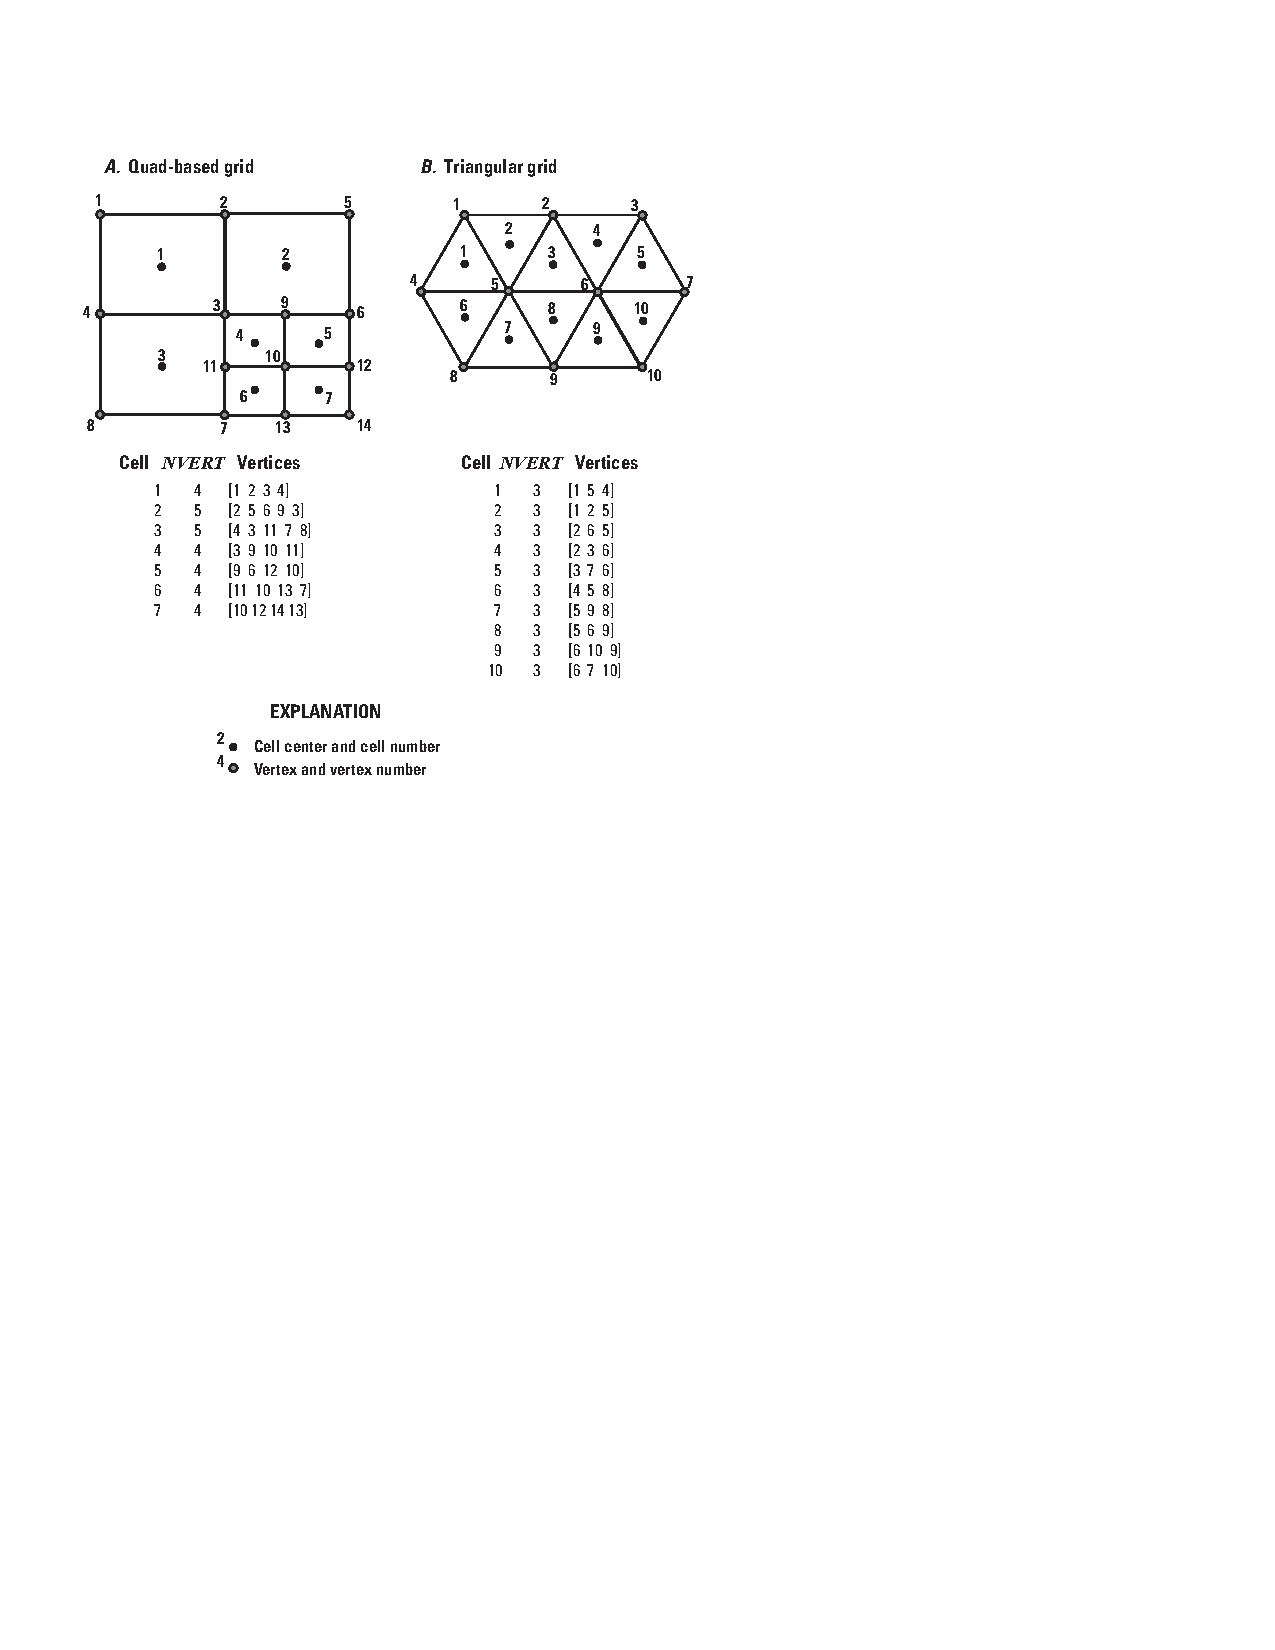
\includegraphics[scale=1.0]{Figures/gwf-fig3-2}
	\caption{Schematic diagram showing the vertices and cells defined using the Discretization by Vertices Package. The list of vertices used to define each cell must be in clockwise order.  From \cite{modflow6gwf}}
	\label{fig:gwf-fig3-2}
\end{figure}


\vspace{5mm}
\subsubsection{Structure of Blocks}
\lstinputlisting[style=blockdefinition]{./mf6ivar/tex/gwf-disv-options.dat}
\lstinputlisting[style=blockdefinition]{./mf6ivar/tex/gwf-disv-dimensions.dat}
\lstinputlisting[style=blockdefinition]{./mf6ivar/tex/gwf-disv-griddata.dat}
\lstinputlisting[style=blockdefinition]{./mf6ivar/tex/gwf-disv-vertices.dat}
\lstinputlisting[style=blockdefinition]{./mf6ivar/tex/gwf-disv-cell2d.dat}

\vspace{5mm}
\subsubsection{Explanation of Variables}
\begin{description}
\input{./mf6ivar/tex/gwf-disv-desc.tex}
\end{description}

\vspace{5mm}
\subsubsection{Example Input File}
\lstinputlisting[style=inputfile]{./mf6ivar/examples/gwf-disv-example.dat}


%\newpage
%\subsection{Unstructured Discretization (DISU) Input File}
%Discretization information for unstructured grids is read from the file that is specified by ``DISU6'' as the file type.  Only one discretization input file (DISU6, DISV6 or DIS6) can be specified for a model.

The shape and position of each cell can be defined using vertices.  This information is optional and is only read if the number of vertices (NVERT) in the DIMENSIONS block is specified and is assigned a value larger than zero.  If the vertices and two-dimensional cell information is provided in this file, then this information is also written to the binary grid file.  Providing this information may be useful for other postprocessing programs that read the binary grid file.

The DISU Package does not support the concept of layers, which is different from the DISU implementation in MODFLOW-USG.  In \mf~all grid input and output for models that use the DISU Package is entered or written as a one-dimensional array of size nodes.

The DISU VERTICES and CELL2D blocks are not required for all simulations.  These blocks are required if the XT3D or the SAVE\_SPECIFIC\_DISCHARGE options are specified in the NPF Package.  In general, it is recommended to include the VERTICES and CELL2D blocks. 

\vspace{5mm}
\subsubsection{Structure of Blocks}
\lstinputlisting[style=blockdefinition]{./mf6ivar/tex/gwf-disu-options.dat}
\lstinputlisting[style=blockdefinition]{./mf6ivar/tex/gwf-disu-dimensions.dat}
\lstinputlisting[style=blockdefinition]{./mf6ivar/tex/gwf-disu-griddata.dat}
\lstinputlisting[style=blockdefinition]{./mf6ivar/tex/gwf-disu-connectiondata.dat}
\lstinputlisting[style=blockdefinition]{./mf6ivar/tex/gwf-disu-vertices.dat}
\lstinputlisting[style=blockdefinition]{./mf6ivar/tex/gwf-disu-cell2d.dat}

\vspace{5mm}
\subsubsection{Explanation of Variables}
\begin{description}
\input{./mf6ivar/tex/gwf-disu-desc.tex}
\end{description}

\vspace{5mm}
\subsubsection{Example Input File}
\lstinputlisting[style=inputfile]{./mf6ivar/examples/gwf-disu-example.dat}



\newpage
\subsection{Initial Conditions (IC) Package}
Initial Conditions (IC) Package information is read from the file that is specified by ``IC6'' as the file type.  Only one IC Package can be specified for a GWE model. 

\vspace{5mm}
\subsubsection{Structure of Blocks}
\lstinputlisting[style=blockdefinition]{./mf6ivar/tex/gwe-ic-options.dat}
\lstinputlisting[style=blockdefinition]{./mf6ivar/tex/gwe-ic-griddata.dat}

\vspace{5mm}
\subsubsection{Explanation of Variables}
\begin{description}
\input{./mf6ivar/tex/gwe-ic-desc.tex}
\end{description}

\vspace{5mm}
\subsubsection{Example Input File}
\lstinputlisting[style=inputfile]{./mf6ivar/examples/gwe-ic-example.dat}



\newpage
\subsection{Output Control (OC) Option}
Input to the Output Control Option of the Surface Water Flow Model is read from the file that is specified as type ``OC6'' in the Name File. If no ``OC6'' file is specified, default output control is used. The Output Control Option determines how and when outflows are printed to the listing file and/or written to a separate binary output file.  Under the default, outflow and overall flow budget are written to the Listing File at the end of every stress period. The default printout format for concentrations is 10G11.4.  The outflow and overall flow budget are also written to the list file if the simulation terminates prematurely due to failed convergence.

\vspace{5mm}
\subsubsection{Structure of Blocks}
\vspace{5mm}

\noindent \textit{FOR EACH SIMULATION}
\lstinputlisting[style=blockdefinition]{./mf6ivar/tex/olf-oc-options.dat}
\vspace{5mm}
\noindent \textit{FOR ANY STRESS PERIOD}
\lstinputlisting[style=blockdefinition]{./mf6ivar/tex/olf-oc-period.dat}

\vspace{5mm}
\subsubsection{Explanation of Variables}
\begin{description}
\input{./mf6ivar/tex/olf-oc-desc.tex}
\end{description}

\vspace{5mm}
\subsubsection{Example Input File}
\lstinputlisting[style=inputfile]{./mf6ivar/examples/olf-oc-example.dat}


\newpage
\subsection{Observation (OBS) Utility for a GWE Model}
GWE & temperature & cellid & -- & Temperature at a specified cell. \\
GWE & flow-ja-face & cellid & cellid & Energy flow in dimensions of energy per time between two adjacent cells.  The energy flow rate includes the contributions from both advection and conduction (including mechanical dispersion) if those packages are active

\newpage
\subsection{Advection (ADV) Package}
Advection (ADV) Package information is read from the file that is specified by ``ADV6'' as the file type.  Only one ADV Package can be specified for a GWT model. 

\vspace{5mm}
\subsubsection{Structure of Blocks}
\lstinputlisting[style=blockdefinition]{./mf6ivar/tex/gwt-adv-options.dat}

\vspace{5mm}
\subsubsection{Explanation of Variables}
\begin{description}
\input{./mf6ivar/tex/gwt-adv-desc.tex}
\end{description}

\vspace{5mm}
\subsubsection{Example Input File}
\lstinputlisting[style=inputfile]{./mf6ivar/examples/gwt-adv-example.dat}



\newpage
\subsection{Conduction and Dispersion (CND) Package}
Conduction and Dispersion (CND) Package information is read from the file that is specified by ``CND6'' as the file type.  Only one CND Package can be specified for a GWE model.  By default, the CND Package uses the mathematical formulation presented for the XT3D option of the NPF Package to represent full three-dimensional anisotropy in groundwater flow.  XT3D can be computationally expensive and can be turned off to use a simplified and approximate form of the dispersion equations that also account for conduction in a heat transport model.  For most problems, however, XT3D will be required to accurately represent conduction and dispersion.

\vspace{5mm}
\subsubsection{Structure of Blocks}
\lstinputlisting[style=blockdefinition]{./mf6ivar/tex/gwe-cnd-options.dat}
\lstinputlisting[style=blockdefinition]{./mf6ivar/tex/gwe-cnd-griddata.dat}

\vspace{5mm}
\subsubsection{Explanation of Variables}
\begin{description}
\input{./mf6ivar/tex/gwe-cnd-desc.tex}
\end{description}

\vspace{5mm}
\subsubsection{Example Input File}
\lstinputlisting[style=inputfile]{./mf6ivar/examples/gwe-cnd-example.dat}



\newpage
\subsection{Energy Storage and Transfer (EST) Package}
Energy Storage and Transfer (EST) Package information is read from the file that is specified by ``EST6'' as the file type.  Only one EST Package can be specified for a GWE model. 

\vspace{5mm}
\subsubsection{Structure of Blocks}
\lstinputlisting[style=blockdefinition]{./mf6ivar/tex/gwe-est-options.dat}
\lstinputlisting[style=blockdefinition]{./mf6ivar/tex/gwe-est-griddata.dat}

\vspace{5mm}
\subsubsection{Explanation of Variables}
\begin{description}
\input{./mf6ivar/tex/gwe-est-desc.tex}
\end{description}

\vspace{5mm}
\subsubsection{Example Input File}
\lstinputlisting[style=inputfile]{./mf6ivar/examples/gwe-est-example.dat}



\newpage
\subsection{Source and Sink Mixing (SSM) Package}
Source and Sink Mixing (SSM) Package information is read from the file that is specified by ``SSM6'' as the file type.  Only one SSM Package can be specified for a GWT model.  The SSM Package is required if the flow model has any stress packages.

The SSM Package is used to add or remove solute mass from GWT model cells based on inflows and outflows from GWF stress packages.  If a GWF stress package provides flow into a model cell, that flow can be assigned a user-specified concentration.  If a GWT stress package removes water from a model cell, the concentration of that water is typically the concentration of the cell, but a ``MIXED'' option is also included so that the user can specify the concentration of that withdrawn water.  This may be useful for representing evapotranspiration, for example.  There are several different ways for the user to specify the concentrations.  

\begin{itemize}
\item The default condition is that sources have a concentration of zero and sinks withdraw water at the calculated concentration of the cell.  This default condition is assigned to any GWF stress package that is not included in a SOURCES block or FILEINPUT block.
\item A second option is to assign auxiliary variables in the GWF model and include a concentration for each stress boundary.  In this case, the user provides the name of the package and the name of the auxiliary variable containing concentration values for each boundary.  As described below for srctype, there are multiple options for defining this behavior.
\item  A third option is to prepare an input file using the \hyperref[sec:spc]{Stress Package Component (SPC6) utility} for any desired GWF stress package.  This SPC6 file allows users to change concentrations by stress period, or to use the time-series option to interpolate concentrations by time step.  This third option was introduced in MODFLOW version 6.3.0.  Information for this approach is entered in an optional FILEINPUT block below.  The SPC6 input file supports list-based concentration input for most corresponding GWF stress packages, but also supports a READASARRAYS array-based input format if a corresponding GWF recharge or evapotranspiration package uses the READASARRAYS option.
\end{itemize}

\noindent The auxiliary method and the SPC6 file input method can both be used for a GWT model, but only one approach can be assigned per GWF stress package.   If a flow package specified in the SOURCES or FILEINPUT blocks is also represented using an advanced transport package (SFT, LKT, MWT, or UZT), then the advanced transport package will override SSM calculations for that package.

\vspace{5mm}
\subsubsection{Structure of Blocks}
\lstinputlisting[style=blockdefinition]{./mf6ivar/tex/gwt-ssm-options.dat}
\lstinputlisting[style=blockdefinition]{./mf6ivar/tex/gwt-ssm-sources.dat}
\vspace{5mm}
\noindent \textit{FILEINPUT BLOCK IS OPTIONAL}
\lstinputlisting[style=blockdefinition]{./mf6ivar/tex/gwt-ssm-fileinput.dat}

\vspace{5mm}
\subsubsection{Explanation of Variables}
\begin{description}
\input{./mf6ivar/tex/gwt-ssm-desc.tex}
\end{description}

\vspace{5mm}
\subsubsection{Example Input File}
\lstinputlisting[style=inputfile]{./mf6ivar/examples/gwt-ssm-example.dat}

% when obs are ready, they should go here


\newpage
\subsection{Constant Temperature (CTP) Package}
Constant Temperature (CTP) Package information is read from the file that is specified by ``CTP6'' as the file type.  Any number of CTP Packages can be specified for a single GWE model, but the same cell cannot be designated as a constant temperature by more than one CTP entry. 

\vspace{5mm}
\subsubsection{Structure of Blocks}
\vspace{5mm}

\noindent \textit{FOR EACH SIMULATION}
\lstinputlisting[style=blockdefinition]{./mf6ivar/tex/gwe-ctp-options.dat}
\lstinputlisting[style=blockdefinition]{./mf6ivar/tex/gwe-ctp-dimensions.dat}
\vspace{5mm}
\noindent \textit{FOR ANY STRESS PERIOD}
\lstinputlisting[style=blockdefinition]{./mf6ivar/tex/gwe-ctp-period.dat}
\gwepackageperioddescription

\vspace{5mm}
\subsubsection{Explanation of Variables}
\begin{description}
\input{./mf6ivar/tex/gwe-ctp-desc.tex}
\end{description}

\vspace{5mm}
\subsubsection{Example Input File}
\lstinputlisting[style=inputfile]{./mf6ivar/examples/gwe-ctp-example.dat}

\vspace{5mm}
\subsubsection{Available observation types}
CTP Package observations are limited to the simulated constant temperature energy flow rate (\texttt{ctp}). The data required for the CTP Package observation type is defined in table~\ref{table:gwe-ctpobstype}. Negative and positive values for an observation represent a loss from and gain to the GWE model, respectively.

\begin{longtable}{p{2cm} p{2.75cm} p{2cm} p{1.25cm} p{7cm}}
\caption{Available CTP Package observation types} \tabularnewline

\hline
\hline
\textbf{Model} & \textbf{Observation type} & \textbf{ID} & \textbf{ID2} & \textbf{Description} \\
\hline
\endhead

\hline
\endfoot

CTP & ctp & cellid or boundname & -- & Energy flow between the groundwater system and a constant-temperature boundary or a group of cells with constant-temperature boundaries.

\label{table:gwe-ctpobstype}
\end{longtable}

\vspace{5mm}
\subsubsection{Example Observation Input File}
\lstinputlisting[style=inputfile]{./mf6ivar/examples/gwe-ctp-example-obs.dat}


\newpage
\subsection{Energy Source Loading (ESL) Package}
Input to the Energy Source Loading (ESL) Package is read from the file that has type ``ESL6'' in the Name File.  Any number of ESL Packages can be specified for a single groundwater energy transport model.

\vspace{5mm}
\subsubsection{Structure of Blocks}
\vspace{5mm}

\noindent \textit{FOR EACH SIMULATION}
\lstinputlisting[style=blockdefinition]{./mf6ivar/tex/gwe-esl-options.dat}
\lstinputlisting[style=blockdefinition]{./mf6ivar/tex/gwe-esl-dimensions.dat}
\vspace{5mm}
\noindent \textit{FOR ANY STRESS PERIOD}
\lstinputlisting[style=blockdefinition]{./mf6ivar/tex/gwe-esl-period.dat}
\gwepackageperioddescription

\vspace{5mm}
\subsubsection{Explanation of Variables}
\begin{description}
\input{./mf6ivar/tex/gwe-esl-desc.tex}
\end{description}

\vspace{5mm}
\subsubsection{Example Input File}
\lstinputlisting[style=inputfile]{./mf6ivar/examples/gwe-esl-example.dat}

\vspace{5mm}
\subsubsection{Available observation types}
Energy Source Loading Package observations include the simulated energy source loading rates (\texttt{esl}). The data required for each ESL Package observation type is defined in table~\ref{table:gwe-eslobstype}. The \texttt{esl} observation is equal to the simulated energy source loading rate. Negative and positive values for an observation represent a loss from and gain to the GWE model, respectively.

\begin{longtable}{p{2cm} p{2.75cm} p{2cm} p{1.25cm} p{7cm}}
\caption{Available ESL Package observation types} \tabularnewline

\hline
\hline
\textbf{Stress Package} & \textbf{Observation type} & \textbf{ID} & \textbf{ID2} & \textbf{Description} \\
\hline
\endhead

\hline
\endfoot

ESL & esl & cellid or boundname & -- & Energy source loading rate between the groundwater system and an energy source loading boundary or a group of boundaries.
\label{table:gwe-eslobstype}
\end{longtable}

\vspace{5mm}
\subsubsection{Example Observation Input File}
\lstinputlisting[style=inputfile]{./mf6ivar/examples/gwe-esl-example-obs.dat}


\newpage
\subsection{Streamflow Energy Transport (SFE) Package}
Streamflow Energy Transport (SFE) Package information is read from the file that is specified by ``SFE6'' as the file type.  There can be as many SFE Packages as necessary for a GWE model. Each SFE Package is designed to work with flows from a corresponding GWF SFR Package. By default \mf uses the SFE package name to determine which SFR Package corresponds to the SFE Package.  Therefore, the package name of the SFE Package (as specified in the GWE name file) must match with the name of the corresponding SFR Package (as specified in the GWF name file).  Alternatively, the name of the flow package can be specified using the FLOW\_PACKAGE\_NAME keyword in the options block.  The GWE SFE Package cannot be used without a corresponding GWF SFR Package.

The SFE Package does not have a dimensions block; instead, dimensions for the SFE Package are set using the dimensions from the corresponding SFR Package.  For example, the SFR Package requires specification of the number of reaches (NREACHES).  SFE sets the number of reaches equal to NREACHES.  Therefore, the PACKAGEDATA block below must have NREACHES entries in it.

\vspace{5mm}
\subsubsection{Structure of Blocks}
\lstinputlisting[style=blockdefinition]{./mf6ivar/tex/gwe-sfe-options.dat}
\lstinputlisting[style=blockdefinition]{./mf6ivar/tex/gwe-sfe-packagedata.dat}
\lstinputlisting[style=blockdefinition]{./mf6ivar/tex/gwe-sfe-period.dat}

\vspace{5mm}
\subsubsection{Explanation of Variables}
\begin{description}
\input{./mf6ivar/tex/gwe-sfe-desc.tex}
\end{description}

\vspace{5mm}
\subsubsection{Example Input File}
\lstinputlisting[style=inputfile]{./mf6ivar/examples/gwe-sfe-example.dat}

\vspace{5mm}
\subsubsection{Available observation types}
Streamflow Energy Transport Package observations include reach temperature and all of the terms that contribute to the continuity equation for each reach. Additional SFE Package observations include energy flow rates for individual reaches, or groups of reaches. The data required for each SFE Package observation type is defined in table~\ref{table:gwe-sfeobstype}. Negative and positive values for \texttt{sfe} observations represent a loss from and gain to the GWE model, respectively. For all other flow terms, negative and positive values represent a loss from and gain from the SFE package, respectively.

\begin{longtable}{p{2cm} p{2.75cm} p{2cm} p{1.25cm} p{7cm}}
\caption{Available SFE Package observation types} \tabularnewline

\hline
\hline
\textbf{Stress Package} & \textbf{Observation type} & \textbf{ID} & \textbf{ID2} & \textbf{Description} \\
\hline
\endfirsthead

\captionsetup{textformat=simple}
\caption*{\textbf{Table \arabic{table}.}{\quad}Available SFE Package observation types.---Continued} \tabularnewline

\hline
\hline
\textbf{Stress Package} & \textbf{Observation type} & \textbf{ID} & \textbf{ID2} & \textbf{Description} \\
\hline
\endhead


\hline
\endfoot

% general APT observations
SFE & temperature & rno or boundname & -- & Reach temperature. If boundname is specified, boundname must be unique for each reach. \\
SFE & flow-ja-face & rno or boundname & rno or -- & Energy flow between two reaches.  If a boundname is specified for ID1, then the result is the total energy flow for all reaches. If a boundname is specified for ID1 then ID2 is not used.\\
SFE & storage & rno or boundname & -- & Simulated energy storage flow rate for a reach or group of reaches. \\
SFE & constant & rno or boundname & -- & Simulated energy constant-flow rate for a reach or group of reaches. \\
SFE & from-mvr & rno or boundname & -- & Simulated energy inflow into a reach or group of reaches from the MVE package. Energy inflow is calculated as the product of provider temperature and the mover flow rate. \\
SFE & to-mvr & rno or boundname & -- & Energy outflow from a reach, or a group of reaches that is available for the MVR package. If boundname is not specified for ID, then the outflow available for the MVR package from a specific reach is observed. \\
SFE & sfe & rno or boundname & -- & Energy flow rate for a reach or group of reaches and its aquifer connection(s). \\

%observations specific to the stream energy transport package
% rainfall evaporation runoff ext-inflow withdrawal outflow
SFE & rainfall & rno or boundname & -- & Rainfall rate applied to a reach or group of reaches multiplied by the rainfall temperature. \\
SFE & evaporation & rno or boundname & -- & Simulated evaporation rate from a reach or group of reaches multiplied by the latent heat of vaporization for determining the amount of energy lost from a reach. \\
SFE & runoff & rno or boundname & -- & Runoff rate applied to a reach or group of reaches multiplied by the runoff temperature. \\
SFE & ext-inflow & rno or boundname & -- & Energy inflow into a reach or group of reaches calculated as the external inflow rate multiplied by the inflow temperature. \\
SFE & ext-outflow & rno or boundname & -- & External outflow from a reach or group of reaches to an external boundary. If boundname is not specified for ID, then the external outflow from a specific reach is observed. In this case, ID is the reach rno. \\
SFE & strmbd-cond & rno or boundname & -- & Amount of heat conductively exchanged with the streambed material. 

\label{table:gwe-sfeobstype}
\end{longtable}

\vspace{5mm}
\subsubsection{Example Observation Input File}
\lstinputlisting[style=inputfile]{./mf6ivar/examples/gwe-sfe-example-obs.dat}




\newpage
\subsection{Lake Energy Transport (LKE) Package}
Lake Energy Transport (LKE) Package information is read from the file that is specified by ``LKE6'' as the file type.  There can be as many LKE Packages as necessary for a GWE model. Each LKE Package is designed to work with flows from a single corresponding GWF LAK Package. By default \mf uses the LKE package name to determine which LAK Package corresponds to the LKE Package.  Therefore, the package name of the LKE Package (as specified in the GWE name file) must match with the name of the corresponding LAK Package (as specified in the GWF name file).  Alternatively, the name of the flow package can be specified using the FLOW\_PACKAGE\_NAME keyword in the options block.  The GWE LKE Package cannot be used without a corresponding GWF LAK Package.

The LKE Package does not have a dimensions block; instead, dimensions for the LKE Package are set using the dimensions from the corresponding LAK Package.  For example, the LAK Package requires specification of the number of lakes (NLAKES).  LKE sets the number of lakes equal to NLAKES.  Therefore, the PACKAGEDATA block below must have NLAKES entries in it.

\vspace{5mm}
\subsubsection{Structure of Blocks}
\lstinputlisting[style=blockdefinition]{./mf6ivar/tex/gwe-lke-options.dat}
\lstinputlisting[style=blockdefinition]{./mf6ivar/tex/gwe-lke-packagedata.dat}
\lstinputlisting[style=blockdefinition]{./mf6ivar/tex/gwe-lke-period.dat}

\vspace{5mm}
\subsubsection{Explanation of Variables}
\begin{description}
\input{./mf6ivar/tex/gwe-lke-desc.tex}
\end{description}

\vspace{5mm}
\subsubsection{Example Input File}
\lstinputlisting[style=inputfile]{./mf6ivar/examples/gwe-lke-example.dat}

\vspace{5mm}
\subsubsection{Available observation types}
Lake Energy Transport Package observations include lake temperature and all of the terms that contribute to the continuity equation for each lake. Additional LKE Package observations include energy flow rates for individual outlets, lakes, or groups of lakes (\texttt{outlet}). The data required for each LKE Package observation type is defined in table~\ref{table:gwe-lkeobstype}. Negative and positive values for \texttt{lke} observations represent a loss from and gain to the GWE model, respectively. For all other flow terms, negative and positive values represent a loss from and gain from the LKE package, respectively.

\begin{longtable}{p{2cm} p{2.75cm} p{2cm} p{1.25cm} p{7cm}}
\caption{Available LKE Package observation types} \tabularnewline

\hline
\hline
\textbf{Stress Package} & \textbf{Observation type} & \textbf{ID} & \textbf{ID2} & \textbf{Description} \\
\hline
\endfirsthead

\captionsetup{textformat=simple}
\caption*{\textbf{Table \arabic{table}.}{\quad}Available LKE Package observation types.---Continued} \tabularnewline

\hline
\hline
\textbf{Stress Package} & \textbf{Observation type} & \textbf{ID} & \textbf{ID2} & \textbf{Description} \\
\hline
\endhead


\hline
\endfoot

% general APT observations
LKE & temperature & lakeno or boundname & -- & Lake temperature. If boundname is specified, boundname must be unique for each lake. \\
LKE & flow-ja-face & lakeno or boundname & lakeno or -- & Energy flow between two lakes connected by an outlet.  If more than one outlet is used to connect the same two lakes, then the energy flow for only the first outlet can be observed.  If a boundname is specified for ID1, then the result is the total energy flow for all outlets for a lake. If a boundname is specified for ID1 then ID2 is not used.\\
LKE & storage & lakeno or boundname & -- & Simulated energy storage flow rate for a lake or group of lakes. \\
LKE & constant & lakeno or boundname & -- & Simulated energy constant-flow rate for a lake or group of lakes. \\
LKE & from-mvr & lakeno or boundname & -- & Simulated energy inflow into a lake or group of lakes from the MVE package. Energy inflow is calculated as the product of provider temperature and the mover flow rate. \\
LKE & to-mvr & outletno or boundname & -- & Energy outflow from a lake outlet, a lake, or a group of lakes that is available for the MVR package. If boundname is not specified for ID, then the outflow available for the MVR package from a specific lake outlet is observed. In this case, ID is the outlet number, which must be between 1 and NOUTLETS. \\
LKE & lke & lakeno or boundname & \texttt{iconn} or -- & Energy flow rate for a lake or group of lakes and its aquifer connection(s). If boundname is not specified for ID, then the simulated lake-aquifer flow rate at a specific lake connection is observed. In this case, ID2 must be specified and is the connection number \texttt{iconn} for lake \texttt{lakeno}. \\

%observations specific to the lake package
% rainfall evaporation runoff ext-inflow withdrawal outflow
LKE & rainfall & lakeno or boundname & -- & Rainfall rate applied to a lake or group of lakes multiplied by the rainfall temperature. \\
LKE & evaporation & lakeno or boundname & -- & Simulated evaporation rate from a lake or group of lakes multiplied by the latent heat of evaporation for determining the energy lost from a lake. \\
LKE & runoff & lakeno or boundname & -- & Runoff rate applied to a lake or group of lakes multiplied by the runoff temperature. \\
LKE & ext-inflow & lakeno or boundname & -- & Energy inflow into a lake or group of lakes calculated as the external inflow rate multiplied by the inflow temperature. \\
LKE & withdrawal & lakeno or boundname & -- & Specified withdrawal rate from a lake or group of lakes multiplied by the simulated lake temperature. \\
LKE & ext-outflow & lakeno or boundname & -- & External outflow from a lake or a group of lakes, through their outlets, to an external boundary.  If the water mover is active, the reported ext-outflow value plus the rate to mover is equal to the total outlet outflow.


\label{table:gwe-lkeobstype}
\end{longtable}

\vspace{5mm}
\subsubsection{Example Observation Input File}
\lstinputlisting[style=inputfile]{./mf6ivar/examples/gwe-lke-example-obs.dat}




\newpage
\subsection{Multi-Aquifer Well Energy Transport (MWE) Package}
Multi-Aquifer Well Energy Transport (MWE) Package information is read from the file that is specified by ``MWE6'' as the file type.  There can be as many MWE Packages as necessary for a GWE model. Each MWE Package is designed to work with flows from a corresponding GWF MAW Package. By default \mf uses the MWE package name to determine which MAW Package corresponds to the MWE Package.  Therefore, the package name of the MWE Package (as specified in the GWE name file) must match with the name of the corresponding MAW Package (as specified in the GWF name file).  Alternatively, the name of the flow package can be specified using the FLOW\_PACKAGE\_NAME keyword in the options block.  The GWE MWE Package cannot be used without a corresponding GWF MAW Package.

The MWE Package does not have a dimensions block; instead, dimensions for the MWE Package are set using the dimensions from the corresponding MAW Package.  For example, the MAW Package requires specification of the number of wells (NMAWWELLS).  MWE sets the number of wells equal to NMAWWELLS.  Therefore, the PACKAGEDATA block below must have NMAWWELLS entries in it.

\vspace{5mm}
\subsubsection{Structure of Blocks}
\lstinputlisting[style=blockdefinition]{./mf6ivar/tex/gwe-mwe-options.dat}
\lstinputlisting[style=blockdefinition]{./mf6ivar/tex/gwe-mwe-packagedata.dat}
\lstinputlisting[style=blockdefinition]{./mf6ivar/tex/gwe-mwe-period.dat}

\vspace{5mm}
\subsubsection{Explanation of Variables}
\begin{description}
\input{./mf6ivar/tex/gwe-mwe-desc.tex}
\end{description}

\vspace{5mm}
\subsubsection{Example Input File}
\lstinputlisting[style=inputfile]{./mf6ivar/examples/gwe-mwe-example.dat}

\vspace{5mm}
\subsubsection{Available observation types}
Multi-Aquifer Well Energy Transport Package observations include well temperature and all of the terms that contribute to the continuity equation for each well. Additional MWE Package observations include energy flow rates for individual wells, or groups of wells; the well volume (\texttt{volume}); and the conductance for a well-aquifer connection conductance (\texttt{conductance}). The data required for each MWE Package observation type is defined in table~\ref{table:gwe-mweobstype}. Negative and positive values for \texttt{mwe} observations represent a loss from and gain to the GWE model, respectively. For all other flow terms, negative and positive values represent a loss from and gain from the MWE package, respectively.

\begin{longtable}{p{2cm} p{2.75cm} p{2cm} p{1.25cm} p{7cm}}
\caption{Available MWE Package observation types} \tabularnewline

\hline
\hline
\textbf{Stress Package} & \textbf{Observation type} & \textbf{ID} & \textbf{ID2} & \textbf{Description} \\
\hline
\endfirsthead

\captionsetup{textformat=simple}
\caption*{\textbf{Table \arabic{table}.}{\quad}Available MWE Package observation types.---Continued} \tabularnewline

\hline
\hline
\textbf{Stress Package} & \textbf{Observation type} & \textbf{ID} & \textbf{ID2} & \textbf{Description} \\
\hline
\endhead


\hline
\endfoot

% general APT observations
MWE & temperature & mawno or boundname & -- & Well temperature. If boundname is specified, boundname must be unique for each well. \\
%flowjaface not included
MWE & storage & mawno or boundname & -- & Simulated energy storage flow rate for a well or group of wells. \\
MWE & constant & mawno or boundname & -- & Simulated energy constant-flow rate for a well or group of wells. \\
MWE & from-mvr & mawno or boundname & -- & Simulated energy inflow into a well or group of wells from the MVE package. Energy inflow is calculated as the product of provider temperature and the mover flow rate. \\
MWE & mwe & mawno or boundname & \texttt{iconn} or -- & Energy flow rate for a well or group of wells and its aquifer connection(s). If boundname is not specified for ID, then the simulated well-aquifer flow rate at a specific well connection is observed. In this case, ID2 must be specified and is the connection number \texttt{iconn} for well \texttt{mawno}. \\

% observations specific to the mwe package
MWE & rate & mawno or boundname & -- & Simulated energy flow rate for a well or group of wells. \\
MWE & fw-rate & mawno or boundname & -- & Simulated energy flow rate for a flowing well or group of flowing wells. \\
MWE & rate-to-mvr & well or boundname & -- & Simulated energy flow rate that is sent to the MVE Package for a well or group of wells.\\
MWE & fw-rate-to-mvr & well or boundname & -- & Simulated energy flow rate that is sent to the MVE Package from a flowing well or group of flowing wells. \\

\label{table:gwe-mweobstype}
\end{longtable}

\vspace{5mm}
\subsubsection{Example Observation Input File}
\lstinputlisting[style=inputfile]{./mf6ivar/examples/gwe-mwe-example-obs.dat}




\newpage
\subsection{Unsaturated-Zone Energy Transport (UZE) Package}
Unsaturated Zone Energy Transport (UZE) Package information is read from the file that is specified by ``UZE6'' as the file type.  There can be as many UZE Packages as necessary for a GWE model. Each UZE Package is designed to work with flows from a corresponding GWF UZF Package. By default \mf uses the UZE package name to determine which UZF Package corresponds to the UZE Package.  Therefore, the package name of the UZE Package (as specified in the GWE name file) must match with the name of the corresponding UZF Package (as specified in the GWF name file).  Alternatively, the name of the flow package can be specified using the FLOW\_PACKAGE\_NAME keyword in the options block.  The GWE UZE Package cannot be used without a corresponding GWF UZF Package.

The UZE Package does not have a dimensions block; instead, dimensions for the UZE Package are set using the dimensions from the corresponding UZF Package.  For example, the UZF Package requires specification of the number of cells (NUZFCELLS).  UZE sets the number of UZE cells equal to NUZFCELLS.  Therefore, the PACKAGEDATA block below must have NUZFCELLS entries in it.  Furthermore, UZE requires the area of each UZE object to equal to the area of the grid cell hosting the corresponding UZF object.  If the area of a UZF object is different than the host grid cell, the GWE model will exit with an error message indicating which cell is in violation of this condition. This check is unique to UZE as UZT does not require the area of the corresponding UZF object to equal the area of the host grid cell.  If this error condition occurs, users should check whether the AUXMULTNAME option in the OPTIONS block of the corresponding UZF input file is activated.  Users could inadvertently circumvent the error check by creating two (or more) UZF objects in the same cell using multiple UZF input packages that each specify a UZF object for the same cell.

\vspace{5mm}
\subsubsection{Structure of Blocks}
\lstinputlisting[style=blockdefinition]{./mf6ivar/tex/gwe-uze-options.dat}
\lstinputlisting[style=blockdefinition]{./mf6ivar/tex/gwe-uze-packagedata.dat}
\lstinputlisting[style=blockdefinition]{./mf6ivar/tex/gwe-uze-period.dat}

\vspace{5mm}
\subsubsection{Explanation of Variables}
\begin{description}
\input{./mf6ivar/tex/gwe-uze-desc.tex}
\end{description}

\vspace{5mm}
\subsubsection{Example Input File}
\lstinputlisting[style=inputfile]{./mf6ivar/examples/gwe-uze-example.dat}

\vspace{5mm}
\subsubsection{Available observation types}
Unsaturated Zone Energy Transport Package observations include UZF cell temperature and all of the terms that contribute to the continuity equation for each UZE cell. Additional UZE Package observations include energy flow rates for individual UZE cells, or groups of UZE cells. The data required for each UZE Package observation type is defined in table~\ref{table:gwe-uzeobstype}. Negative and positive values for \texttt{uzt} observations represent a loss from and gain to the GWE model, respectively. For all other flow terms, negative and positive values represent a loss from and gain from the UZE package, respectively.

\begin{longtable}{p{2cm} p{2.75cm} p{2cm} p{1.25cm} p{7cm}}
\caption{Available UZE Package observation types} \tabularnewline

\hline
\hline
\textbf{Stress Package} & \textbf{Observation type} & \textbf{ID} & \textbf{ID2} & \textbf{Description} \\
\hline
\endfirsthead

\captionsetup{textformat=simple}
\caption*{\textbf{Table \arabic{table}.}{\quad}Available UZE Package observation types.---Continued} \tabularnewline

\hline
\hline
\textbf{Stress Package} & \textbf{Observation type} & \textbf{ID} & \textbf{ID2} & \textbf{Description} \\
\hline
\endhead


\hline
\endfoot

% general APT observations
UZE & temperature & uzeno or boundname & -- & uze cell temperature. If boundname is specified, boundname must be unique for each uze cell. \\
UZE & flow-ja-face & uzeno or boundname & uzeno or -- & Energy flow between two uze cells.  If a boundname is specified for ID1, then the result is the total energy flow for all uze cells. If a boundname is specified for ID1 then ID2 is not used.\\
UZE & storage & uzeno or boundname & -- & Simulated energy storage flow rate for a uze cell or group of uze cells. \\
UZE & constant & uzeno or boundname & -- & Simulated energy constant-flow rate for a uze cell or a group of uze cells. \\
UZE & from-mvr & uzeno or boundname & -- & Simulated energy inflow into a uze cell or group of uze cells from the MVE package. Energy inflow is calculated as the product of provider temperature and the mover flow rate. \\
UZE & uze & uzeno or boundname & -- & Energy flow rate for a uze cell or group of uze cells and its aquifer connection(s). \\

%observations specific to the uze package
% infiltration rej-inf uzet rej-inf-to-mvr
UZE & infiltration & uzeno or boundname & -- & Infiltration rate applied to a uze cell or group of uze cells multiplied by the infiltration temperature. \\
UZE & rej-inf & uzeno or boundname & -- & Rejected infiltration rate applied to a uze cell or group of uze cells multiplied by the infiltration temperature. \\
UZE & uzet & uzeno or boundname & -- & Unsaturated zone evapotranspiration rate applied to a uze cell or group of uze cells multiplied by the uze cell temperature. \\
UZE & rej-inf-to-mvr & uzeno or boundname & -- & Rejected infiltration rate applied to a uze cell or group of uze cells multiplied by the infiltration temperature that is sent to the mover package. \\

\label{table:gwe-uzeobstype}
\end{longtable}

\vspace{5mm}
\subsubsection{Example Observation Input File}
\lstinputlisting[style=inputfile]{./mf6ivar/examples/gwe-uze-example-obs.dat}




\newpage
\subsection{Flow Model Interface (FMI) Package}
Flow Model Interface (FMI) Package information is read from the file that is specified by ``FMI6'' as the file type.  The FMI Package file is required only if the PRT Model is running in a separate simulation from a previously run GWF Model. If the PRT Model is coupled to a GWF Model by an exchange, the FMI Package file is not required. Only one FMI Package can be specified for a PRT model.

The PRT Model needs groundwater flows for model grid cells, for boundary conditions, and for other terms, such as the flow of water in or out of storage.  The FMI Package is the interface between the PRT Model and simulated groundwater flows provided by a corresponding GWF Model that is running concurrently within the simulation or from binary budget files that were created from a previous GWF model run.  The following are several different FMI simulation cases:

\begin{itemize}

\item Flows are provided by a corresponding GWF Model running in the same simulation---in this case, all groundwater flows are calculated by the corresponding GWF Model and provided through FMI to the transport model.  This is a common use case in which the user wants to run the flow and particle-tracking models as part of a single simulation.  The GWF and PRT models must be part of a GWF-PRT Exchange that is listed in mfsim.nam.  If a GWF-PRT Exchange is specified by the user, then the user does not need to specify an FMI Package input file for the simulation, unless an FMI option is needed.  If a GWF-PRT Exchange is specified and the FMI Package is specified, then the PACKAGEDATA block below is not read or used.

\item Flows are provided from a previous GWF model simulation---in this case FMI should be provided in the PRT name file and the head and budget files should be listed in the FMI PACKAGEDATA block.  In this case, FMI reads the simulated head and flows from these files and makes them available to the particle-tracking model.  There are some additional considerations when the heads and flows are provided from binary files.

\begin{itemize}
\item The binary budget file must contain the simulated flows for all of the packages that were included in the GWF model run.  Saving of flows can be activated for all packages by specifying ``SAVE\_FLOWS'' as an option in the GWF name file.  The GWF Output Control Package must also have ``SAVE BUDGET ALL'' specified.  The easiest way to ensure that all flows and heads are saved is to use the following simple form of a GWF Output Control file:

\begin{verbatim}
BEGIN OPTIONS
  HEAD FILEOUT mymodel.hds
  BUDGET FILEOUT mymodel.bud
END OPTIONS

BEGIN PERIOD 1
  SAVE HEAD ALL
  SAVE BUDGET ALL
END PERIOD
\end{verbatim}

\item The binary budget file must have the same number of budget terms listed for each time step.  This will always be the case when the binary budget file is created by \mf.
\item The binary heads file must have heads saved for all layers in the model.  This will always be the case when the binary head file is created by \mf.  This was not always the case as previous MODFLOW versions allowed different save options for each layer.
\item If the binary budget and head files have more than one time step for a single stress period, then the budget and head information must be contained within the binary file for every time step in the simulation stress period.
\item The binary budget and head files must correspond in terms of information stored for each time step and stress period.
\item If the binary budget and head files have information provided for only the first time step of a given stress period, this information will be used for all time steps in that stress period in the PRT simulation. If the final (or only) stress period in the binary budget and head files contains data for only one time step, this information will be used for any subsequent time steps and stress periods in the PRT simulation. This makes it possible to provide flows, for example, from a steady-state GWF stress period and have those flows used for all PRT time steps in that stress period, for all remaining time steps in the PRT simulation, or for all time steps throughout the entire PRT simulation. With this option, it is possible to have smaller time steps in the PRT simulation than the time steps used in the GWF simulation. Note that this cannot be done when the GWF and PRT models are run in the same simulation, because in that case, both models are solved over the same sequence of time steps and stress periods, as listed in the TDIS Package. The option to read flows from a previous GWF simulation via Flow Model Interface may offer an efficient alternative to running both models in the same simulation, but comes at the cost of having potentially very large budget files.
\item The binary grid file is optional but recommended, as it allows \mf to verify that the GWF and PRT model grids are identical.
\end{itemize}

\end{itemize}

\noindent Determination of which FMI use case to invoke requires careful consideration of the different advantages and disadvantages of each case.  For example, running PRT and GWF in the same simulation can often be faster because GWF flows are passed through memory to the PRT model instead of being written to files.  The disadvantage of this approach is that the same time step lengths must be used for both GWF and PRT.  Ultimately, it should be relatively straightforward to test different ways in which GWF and PRT interact and select the use case most appropriate for the particular problem. 

\vspace{5mm}
\subsubsection{Structure of Blocks}
\lstinputlisting[style=blockdefinition]{./mf6ivar/tex/prt-fmi-packagedata.dat}

\vspace{5mm}
\subsubsection{Explanation of Variables}
\begin{description}
\input{./mf6ivar/tex/prt-fmi-desc.tex}
\end{description}

\vspace{5mm}
\subsubsection{Example Input File}
\lstinputlisting[style=inputfile]{./mf6ivar/examples/prt-fmi-example.dat}



\newpage
\subsection{Mover Energy Transport (MVE) Package}
Mover Energy Transport (MVE) Package information is read from the file that is specified by ``MVE6'' as the file type.  Only one MVE Package can be specified for a GWE model.  

The MVE Package is used to route thermal energy according to flows from the GWF Water Mover (MVR) Package.  The MVE Package must be activated by the user if the MVR Package is active in the corresponding the GWF Model.  Flows from the GWF MVR Package must be available to the GWE model either through activation of a GWF-GWE Exchange or through specification of ``GWFMOVER'' in the PACKAGEDATA block of the GWE FMI Package.  

\vspace{5mm}
\subsubsection{Structure of Blocks}
\lstinputlisting[style=blockdefinition]{./mf6ivar/tex/gwe-mve-options.dat}

\vspace{5mm}
\subsubsection{Explanation of Variables}
\begin{description}
\input{./mf6ivar/tex/gwe-mve-desc.tex}
\end{description}

\vspace{5mm}
\subsubsection{Example Input File}
\lstinputlisting[style=inputfile]{./mf6ivar/examples/gwe-mve-example.dat}



\newpage
\subsection{Groundwater Energy Transport (GWE) Exchange}
Input to the Groundwater Energy Transport (GWE-GWE) Exchange is read from the file that has type ``GWE6-GWE6'' in the Simulation Name File.

The list of exchanges entered into the EXCHANGEDATA block must be identical to the list of exchanges entered for the GWF-GWF input file.  One way to ensure that this information is identical is to put this list into an external file and refer to this same list using the OPEN/CLOSE functionality in both this EXCHANGEDATA input block and the EXCHANGEDATA input block in the GWF-GWF input file.

\vspace{5mm}
\subsubsection{Structure of Blocks}
\lstinputlisting[style=blockdefinition]{./mf6ivar/tex/exg-gwegwe-options.dat}
\lstinputlisting[style=blockdefinition]{./mf6ivar/tex/exg-gwegwe-dimensions.dat}
\lstinputlisting[style=blockdefinition]{./mf6ivar/tex/exg-gwegwe-exchangedata.dat}

\vspace{5mm}
\subsubsection{Explanation of Variables}
\begin{description}
\input{./mf6ivar/tex/exg-gwegwe-desc.tex}
\end{description}

\vspace{5mm}
\subsubsection{Example Input File}
\lstinputlisting[style=inputfile]{./mf6ivar/examples/exg-gwegwe-example.dat}

\vspace{5mm}
\subsubsection{Available observation types}
GWE-GWE Exchange observations include the simulated flow for any exchange (\texttt{flow-ja-face}). The data required for each GWE-GWE Exchange observation type is defined in table~\ref{table:gwe-gweobstype}. For \texttt{flow-ja-face} observation types, negative and positive values represent a loss from and gain to the first model specified for this exchange.

\begin{longtable}{p{2cm} p{2.75cm} p{2cm} p{1.25cm} p{7cm}}
\caption{Available GWE-GWE Exchange observation types} \tabularnewline

\hline
\hline
\textbf{Exchange} & \textbf{Observation type} & \textbf{ID} & \textbf{ID2} & \textbf{Description} \\
\hline
\endhead

\hline
\endfoot

GWE-GWE & flow-ja-face & exchange number or boundname & -- & Energy flow between model 1 and model 2 for a specified exchange (which is the consecutive exchange number listed in the EXCHANGEDATA block), or the sum of these exchange flows by boundname if boundname is specified.
\label{table:gwe-gweobstype}
\end{longtable}


\vspace{5mm}
\subsubsection{Example Observation Input File}
\lstinputlisting[style=inputfile]{./mf6ivar/examples/exg-gwegwe-example-obs.dat}



